\documentclass[11pt]{article}
\usepackage[margin=1in]{geometry}
\usepackage{amsmath,amssymb,bm}
\usepackage{booktabs,graphicx,xcolor,array}
\usepackage[most]{tcolorbox}
\usepackage{tikz}
\usetikzlibrary{arrows.meta,decorations.pathreplacing,calc}
\usepackage[hidelinks]{hyperref}
\usepackage{enumitem}
\setlist{itemsep=2pt,topsep=4pt}

\newcommand{\um}{\,\mu\mathrm{m}}
\newcommand{\J}{\mathcal{J}}
\newcommand{\A}{\mathsf{A}}
\newcommand{\Hm}{\mathsf{H}}
\newcommand{\N}{\mathbf{N}}
\newcommand{\bpsi}{\bm{\psi}}
\newcommand{\bmu}{\bm{\mu}}
\newcommand{\Fin}{F_{\mathrm{in}}}
\newcommand{\seq}{s_{\mathrm{eq}}}
\newcommand{\dd}{\mathrm{d}}
\newcommand{\rdet}{r_{\mathrm{det}}}
\tcbset{mybox/.style={colback=gray!4,colframe=gray!55,boxrule=0.5pt,arc=2pt,left=6pt,right=6pt,top=4pt,bottom=4pt}}

\title{\textbf{Estimating $D_x$ from Noisy Droplet Counts}\\[4pt]
\large Sampling noise, the Poisson loss, and error bars\\ for the steady-state problem}
\date{October 2026}
\author{}

\graphicspath{{figures/}}

\begin{document}
\maketitle
\vspace{-2em}
\tableofcontents

%==================================================================
\section{From exact data to counted droplets}
%==================================================================
In the noise-free experiment, the data were the model's exact size distribution, and the method recovered the true diffusivity $D_x$ to about nine digits. Real measurements are not like that. An instrument looks at a small volume of chamber air and \emph{counts} the droplets it finds there, sorted into size bins. This note adds that one ingredient, \textbf{sampling noise}, and works out what changes.

\paragraph{Why counting creates noise.} We assume the chamber is \emph{well mixed}: on average, every part of it contains the same size distribution. So a sample taken anywhere is representative \emph{on average}. But a small sample contains only a limited number of droplets, and exactly how many of each size happen to be inside it at that moment is a matter of chance. A poll is a good analogy: if people are thoroughly mixed, a random poll is unbiased, but a poll of 20 people still gives noticeably different answers each time. Well-mixed removes \emph{bias}; it does not remove this luck-of-the-draw \emph{noise}.

\paragraph{When it matters.} The noise is large when samples are small or bins are sparsely populated, as with instrument data, especially for the rare large droplets. It is negligible when a sample contains an enormous number of droplets, as when a simulation reports every droplet in its domain.

\paragraph{What changes.} Very little of the machinery: the model, the adjoint, and the optimizer are the same as before. The loss changes, and so does one vector in the adjoint calculation. The bigger change is in the \emph{question}. With noisy data we cannot recover $D_x$ exactly, so the goal becomes an estimate \emph{with an honest error bar}. Sections~\ref{sec:obs}--\ref{sec:errorbar} develop the theory; Section~\ref{sec:experiments} tests it.

%==================================================================
\section{The model}\label{sec:model}
%==================================================================
We describe droplet sizes by $x = r^2$ ($\mu$m$^2$). The size distribution $N(x)$ (cm$^{-3}\,\mu$m$^{-2}$) is defined so that $N(x)\,\dd x$ is the number of droplets per cm$^3$ of air with $r^2$ between $x$ and $x+\dd x$. In a steady, well-mixed chamber it satisfies
\begin{equation}\label{eq:fp}
\frac{\dd F}{\dd x} + \lambda(x)\,N = 0,\qquad F = A(x)\,N - D_x\,\frac{\dd N}{\dd x},\qquad F(x_{\min}) = \Fin,\quad F(x_{\max}) = 0 .
\end{equation}
Here $F$ is the flux of droplets through size $x$; $A(x) = a\,(s - \seq(r))$ is the condensational growth rate, with Köhler equilibrium supersaturation $\seq = A_k/r - B_k/r^3$; $D_x$ is the turbulent broadening we want to estimate; $\lambda(x) = kx$ is the rate at which droplets fall out; and $\Fin = 100$ cm$^{-3}$s$^{-1}$ is the rate at which new droplets are injected at the smallest size.

We solve \eqref{eq:fp} with finite volumes: $n = 8000$ equal cells of width $\Delta x = 0.1125\um^2$, spanning $r$ from $0.0325$ to $30\um$, with Scharfetter--Gummel fluxes between cells. The result is a tridiagonal linear system
\begin{equation}\label{eq:system}
\A(D_x)\,\N = \mathbf{b},\qquad \mathbf{b} = (\Fin,0,\dots,0)^\top,
\end{equation}
where $N_i$ is the average of $N(x)$ over cell $i$, so $N_i\,\Delta x$ is the concentration of droplets in that cell. Parameter values are in Appendix~\ref{app:params}.

%==================================================================
\section{What the instrument sees}\label{sec:obs}
%==================================================================
\subsection{Sample volume, bins, and expected counts}
The instrument examines a volume $V$ (cm$^3$) of chamber air and counts the droplets in each size bin $[x_k, x_{k+1}]$, $k = 1,\dots,K$. The data are whole numbers,
\[
c_k = \text{number of droplets counted in bin } k .
\]
For simplicity we make each bin exactly $m$ consecutive model cells, so bin edges always fall on cell edges (Figure~\ref{fig:bins}). We use $m = 8$, giving $K = 1000$ bins of width $0.9\um^2$.

Because the chamber is well mixed, the expected number of droplets in the sample is the sample volume times the concentration. For bin $k$,
\begin{equation}\label{eq:mu}
\mu_k = V\int_{x_k}^{x_{k+1}} N(x)\,\dd x = V\,\Delta x\sum_{i\,\in\,\text{bin }k} N_i ,
\qquad\text{or}\qquad \bmu = V\,\Hm\,\N .
\end{equation}
Units: cm$^3$ $\times$ cm$^{-3}\mu$m$^{-2}$ $\times$ $\mu$m$^2$ is a pure number, a count. The matrix $\Hm$ adds $N_i\,\Delta x$ over the cells of each bin; if each bin were a single cell ($m=1$), the sum would have one term and $\Hm = \Delta x\,\mathsf{I}$. Note that $\mu_k$ is an \emph{average}: an actual sample contains more or fewer droplets than $\mu_k$ by chance.

The sample volume sets how many droplets are counted in total, $V\sum_i N_i\,\Delta x$. With the reference concentration of about $20{,}600$ cm$^{-3}$ (for $D_x = 10$), samples of $V = 0.01$, $0.1$ and $1$ cm$^3$ hold about $200$, $2000$ and $20{,}000$ droplets. Figure~\ref{fig:samples} shows what such samples look like.

\begin{figure}[h]
\centering
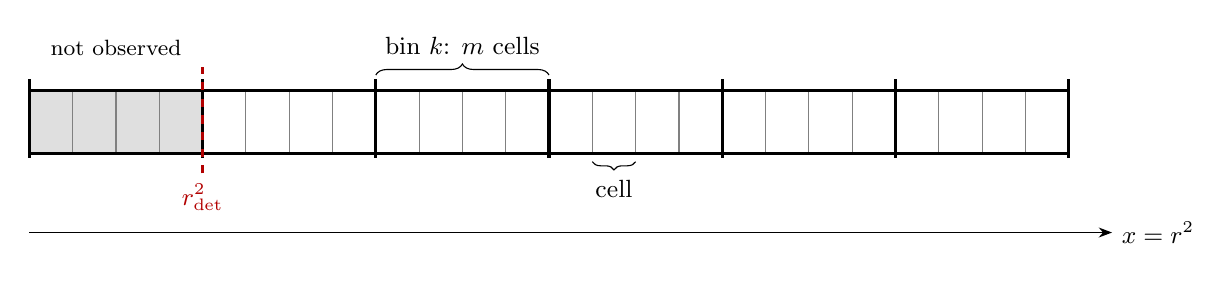
\begin{tikzpicture}[x=0.55cm,y=1cm,every node/.style={font=\small}]
\fill[gray!25] (0,0) rectangle (4,0.8);
\foreach \i in {0,...,23}{\draw[gray] (\i,0) rectangle ++(1,0.8);}
\foreach \j in {0,4,8,12,16,20,24}{\draw[very thick] (\j,-0.05) -- (\j,0.95);}
\draw[very thick] (0,0) -- (24,0); \draw[very thick] (0,0.8) -- (24,0.8);
\node[align=center,font=\footnotesize] at (2,1.35) {not observed};
\draw[decorate,decoration={brace,amplitude=4pt}] (8,1.0) -- (12,1.0) node[midway,above=4pt] {bin $k$: $m$ cells};
\draw[decorate,decoration={brace,amplitude=3pt,mirror}] (13,-0.1) -- (14,-0.1) node[midway,below=3pt] {cell};
\draw[red!70!black,dashed,thick] (4,-0.25) -- (4,1.1);
\node[red!70!black] at (4,-0.55) {$\rdet^2$};
\draw[-{Stealth}] (0,-1.0) -- (25,-1.0) node[right] {$x = r^2$};
\end{tikzpicture}
\caption{Model cells (thin lines) grouped into observation bins of $m$ cells (thick lines). Cells below the detection limit (shaded) belong to no observed bin.}\label{fig:bins}
\end{figure}

\begin{figure}[h]
\centering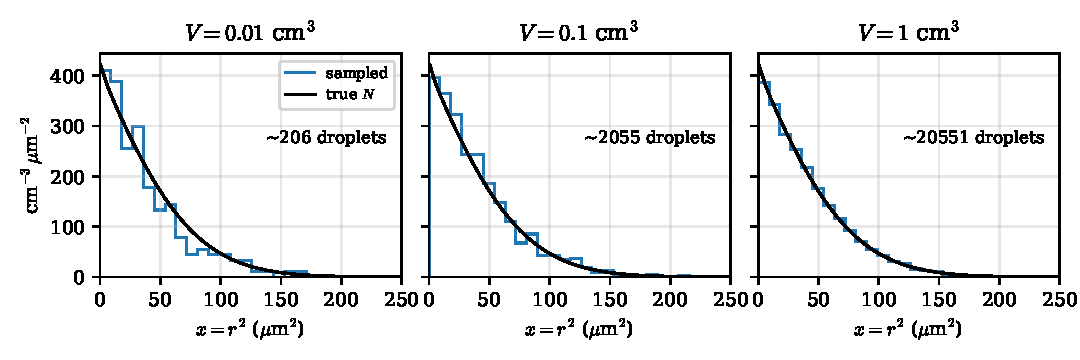
\includegraphics[width=\textwidth]{f_samples.pdf}
\caption{One random sample at each of three sample volumes (true $D_x = 10$), converted back to concentration (counts divided by $V$ and bin width) and compared with the true $N$. For display only, these use wider bins of 80 cells. Small samples are visibly noisy, especially in the tail.}\label{fig:samples}
\end{figure}

\subsection{The detection limit: unobserved is not the same as zero}
Real instruments cannot see droplets smaller than some radius $\rdet$. It's tempting to treat those bins as ``observed, zero droplets.'' That would be wrong. There \emph{are} plenty of droplets there; we simply did not look. Recording zeros would tell the fit ``we looked and found nothing,'' and the fit would distort $D_x$ to suppress small droplets.

The correct treatment is to \textbf{leave those bins out of the data entirely}. The model still covers the full size range, because small droplets exist and feed the larger ones. Only the bins lying entirely above $\rdet$ are compared with data (Figure~\ref{fig:bins}).

%==================================================================
\section{How the counts are distributed}\label{sec:stats}
%==================================================================
\subsection{One bin: the Poisson distribution}
Suppose the chamber holds $M$ droplets in bin $k$. Because the chamber is well mixed, each of them is inside the sampled volume with the same small probability $q = V/V_{\mathrm{chamber}}$, independently of the others. Counting how many land in the sample is like flipping $M$ coins that each come up heads with probability $q$. The count is therefore \emph{binomial}:
\[
P(c) = \binom{M}{c}\,q^c\,(1-q)^{M-c},\qquad \text{with mean } Mq = \mu_k .
\]
In a chamber, $M$ is enormous and $q$ is tiny (cubic centimeters out of cubic meters). Let $M\to\infty$ and $q\to0$ with $Mq = \mu$ held fixed, and look at the pieces one at a time:
\[
\binom{M}{c}q^c(1-q)^{M-c}
= \underbrace{\frac{M(M-1)\cdots(M-c+1)}{M^c}}_{\to\,1}\cdot\frac{\mu^c}{c!}\cdot\underbrace{\Bigl(1-\frac{\mu}{M}\Bigr)^{M}}_{\to\,e^{-\mu}}\cdot\underbrace{\Bigl(1-\frac{\mu}{M}\Bigr)^{-c}}_{\to\,1}.
\]
The limit is the \textbf{Poisson distribution}:
\begin{equation}\label{eq:poisson}
P(c_k\mid D_x) = \frac{\mu_k^{\,c_k}\,e^{-\mu_k}}{c_k!},\qquad c_k = 0,1,2,\dots
\end{equation}
The model enters only through the expected count $\mu_k$. The Poisson distribution has a key property: \textbf{its variance equals its mean}. A bin expecting $\mu$ droplets typically misses by about $\sqrt\mu$, so the \emph{relative} error is $1/\sqrt\mu$ (Figure~\ref{fig:poisson}). A bin expecting $10{,}000$ droplets is accurate to about $1\%$; a bin expecting $4$, only to about $50\%$.

\begin{figure}[h]
\centering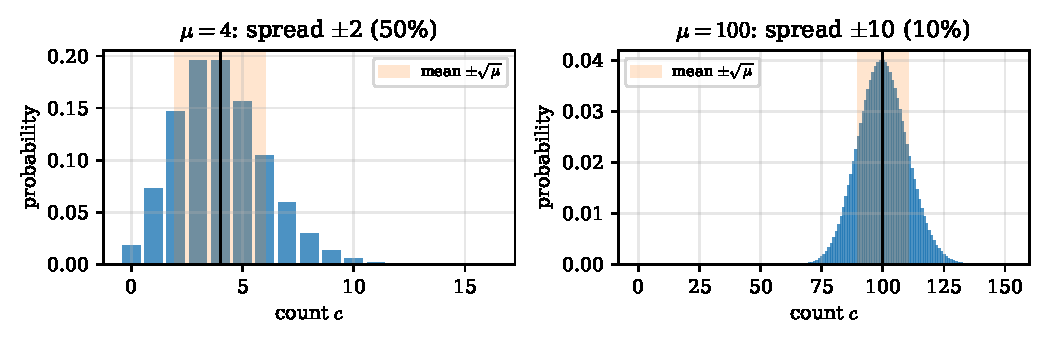
\includegraphics[width=\textwidth]{f_poisson.pdf}
\caption{Poisson distributions with expected counts $4$ and $100$. The typical deviation is $\sqrt\mu$, so relative noise shrinks as counts grow.}\label{fig:poisson}
\end{figure}

\subsection{Many bins: independence}
Different bins count different droplets, and in the same limit their counts are \emph{independent}. Formally: if the total count is Poisson and each droplet independently falls in bin $k$ with some probability, the bin counts are independent Poisson variables.

It's worth separating two ideas that are easy to confuse:
\begin{itemize}
\item \textbf{Neighboring bins have similar counts.} True, but that is about the \emph{expected} counts: the true distribution is smooth, so neighboring $\mu_k$ are similar. The model already accounts for this.
\item \textbf{Neighboring bins have correlated \emph{errors}.} This is what independence rules out. If two bins each expect 100 droplets and one happens to get 115, under the Poisson model that says nothing about whether the other gets more or less than 100.
\end{itemize}
Correlated errors do appear in real data when something \emph{shared} shifts many bins at once: the sample happens to come from a pocket of air with more droplets, the chamber's supersaturation is momentarily high so the whole distribution shifts, or the sample volume is slightly wrong. These make real counts more variable than Poisson predicts. They are physics and instrument effects beyond pure sampling, and we leave them for later. In the synthetic experiments here, independence holds exactly, because we draw each bin's count independently.

%==================================================================
\section{The loss function}\label{sec:loss}
%==================================================================
\subsection{Derivation}
\paragraph{Likelihood.} By independence, the probability of the whole observed histogram is a product over the observed bins:
\[
L(D_x) = \prod_{k\,\in\,\mathrm{obs}}\frac{\mu_k^{\,c_k}\,e^{-\mu_k}}{c_k!}.
\]
Read as a function of $D_x$ with the data fixed, this is the \textbf{likelihood}: how probable the observed counts would be if the true diffusivity were $D_x$. The natural estimate is the value that makes the data most probable, the \textbf{maximum-likelihood estimate}.

\paragraph{Negative log-likelihood.} Maximizing $L$ is the same as minimizing $-\ln L$ (the logarithm is increasing), which turns the product into a sum:
\[
-\ln L = \sum_{k\,\in\,\mathrm{obs}}\bigl[\mu_k - c_k\ln\mu_k + \ln c_k!\bigr].
\]
The last term depends only on the data, not on $D_x$, so we can drop it.

\paragraph{Subtract the best possible fit.} If each $\mu_k$ could be chosen freely, a term would be smallest where $\frac{\dd}{\dd\mu}(\mu - c\ln\mu) = 1 - c/\mu = 0$, i.e.\ at $\mu = c$. Subtracting this best-possible value and multiplying by 2 gives the \textbf{Poisson deviance}, which we use as the loss:
\begin{equation}\label{eq:dev}
\boxed{\;\J(\ell) = 2\sum_{k\,\in\,\mathrm{obs}}\left[c_k\ln\frac{c_k}{\mu_k(\ell)} - c_k + \mu_k(\ell)\right],\qquad 0\ln0\equiv0,\qquad \ell = \ln D_x.\;}
\end{equation}
The subtracted piece doesn't depend on $D_x$, so $\J$ has the same minimizer as $-\ln L$. The factor 2 makes the curvature formula of Section~\ref{sec:errorbar} simple. As before, we estimate $\ell = \ln D_x$, so $D_x$ stays positive and changes are measured as ratios.

\subsection{Properties}
\begin{itemize}
\item \textbf{Never negative; zero only for a perfect fit.} For fixed $c\ge0$, the term $f(\mu) = c\ln(c/\mu) - c + \mu$ has $f'(\mu) = 1 - c/\mu$ and $f''(\mu) = c/\mu^2\ge0$. So it is convex, with its minimum $f(c) = 0$ at $\mu = c$. Hence $\J\ge0$, with equality only when every $\mu_k = c_k$. With noisy data, even the true $D_x$ cannot match random counts exactly, so the loss at the minimum is positive.
\item \textbf{Empty bins are handled correctly.} A bin with $c_k = 0$ contributes $2\mu_k$, penalizing the model for predicting droplets that weren't seen.
\item \textbf{Relation to least squares.} When counts are large, write $c = \mu + \varepsilon$ and expand $\ln(1 + \varepsilon/\mu)$ to second order:
\[
2\Bigl[(\mu+\varepsilon)\ln\Bigl(1+\frac{\varepsilon}{\mu}\Bigr) - \varepsilon\Bigr] \approx \frac{(c-\mu)^2}{\mu}.
\]
So the deviance is \emph{weighted} least squares, with each bin weighted by $1/\mu_k$, the inverse of its noise variance. Plain least squares, used in the noise-free experiment, treats every bin as equally reliable. It lets the high-count bins near the peak dominate and nearly ignores the sparse tail bins, where much of the broadening signal lives. The exact form \eqref{eq:dev} remains correct for bins with only a few counts, where this approximation fails.
\end{itemize}

%==================================================================
\section{The gradient and the optimizer}\label{sec:gradient}
%==================================================================
The adjoint method needs only $\mathbf{g} = \partial\J/\partial\N$. Differentiating \eqref{eq:dev} and using $\bmu = V\Hm\N$:
\begin{equation}\label{eq:g}
\frac{\partial\J}{\partial\mu_k} = 2\Bigl(1 - \frac{c_k}{\mu_k}\Bigr)
\quad\Longrightarrow\quad
\mathbf{g} = V\,\Hm^\top\Bigl[\,2\bigl(1 - c_k/\mu_k\bigr)\Bigr]_k ,
\end{equation}
with zero for unobserved bins. In words: each cell receives its bin's residual weight $2(1 - c_k/\mu_k)$, times $V\Delta x$. The weight is zero where the model matches the count, positive where it predicts too many droplets, and negative where it predicts too few. Everything else is unchanged from the noise-free case:
\begin{equation}\label{eq:adjoint}
\A^\top\bpsi = -\mathbf{g},\qquad \frac{d\J}{dD_x} = \bpsi^\top\frac{d\A}{dD_x}\N,\qquad \frac{d\J}{d\ell} = D_x\,\frac{d\J}{dD_x}.
\end{equation}
Cells below the detection limit get $g_i = 0$, but they still take part in the adjoint solve, so the gradient correctly accounts for how they feed the observed sizes.

\begin{tcolorbox}[mybox,title={\textbf{Loss and gradient for noisy counts}}]
\begin{enumerate}[leftmargin=*,label=\arabic*.]
\item $D_x = e^\ell$. Solve $\A\N = \mathbf{b}$.
\item Expected counts $\mu_k = V\Delta x\sum_{i\in k}N_i$; loss $\J$ from \eqref{eq:dev} over observed bins.
\item $\mathbf{g}$ from \eqref{eq:g}; adjoint solve $\A^\top\bpsi = -\mathbf{g}$, reusing the factorization of $\A$.
\item Return $\J$ and $d\J/d\ell = D_x\,\bpsi^\top(d\A/dD_x)\N$.
\end{enumerate}
\end{tcolorbox}

\paragraph{Optimizer.} We use the same gradient descent as in the noise-free case: a step size estimated from the last two gradients, a cap of one unit in $\ell$ per iteration, and backtracking until the loss decreases. Three small changes:
\begin{itemize}
\item \textbf{Bounds.} $D_x$ is restricted to $[10^{-3}, 10^{3}]\um^4$/s. With very little data, the best fit can wander far off.
\item \textbf{A looser stopping rule.} Stop when $|d\J/d\ell| < 10^{-7}$. There is no point chasing digits far beyond the statistical precision.
\item \textbf{No normalization.} The loss is not divided by anything.
\end{itemize}
Every fit starts from $D_x = 1$.

%==================================================================
\section{Error bars from a single sample}\label{sec:errorbar}
%==================================================================
With noise, each new sample gives a slightly different estimate $\hat\ell$. With synthetic data we can simply repeat the experiment many times and measure the scatter directly (Section~\ref{sec:mc}). With real data we usually have one sample, so we need an error bar from that sample alone.

\paragraph{The idea.} Near its minimum, the loss is approximately a parabola in $\ell$:
\[
\J(\ell) \approx \J(\hat\ell) + \tfrac12\,\J''(\hat\ell)\,(\ell - \hat\ell)^2 .
\]
Since $\J = 2(-\ln L) + \text{const}$, the likelihood is then approximately
\[
L(\ell) \propto e^{-\J(\ell)/2} \propto \exp\!\Bigl(-\frac{(\ell - \hat\ell)^2}{2\,\sigma^2}\Bigr),\qquad \sigma^2 = \frac{2}{\J''(\hat\ell)} .
\]
This is a Gaussian (bell curve) in $\ell$ centered at the estimate, with standard deviation $\sigma$. A sharply curved loss means the data pin $\ell$ down tightly; a flat loss means they don't. So the error bar is
\begin{equation}\label{eq:sd}
\boxed{\;\mathrm{sd}(\hat\ell) \approx \sqrt{\frac{2}{\J''(\hat\ell)}}\;}
\end{equation}
We compute $\J''$ by finite-differencing the adjoint gradient: $\J''\approx[g(\hat\ell + h) - g(\hat\ell - h)]/(2h)$ with $h = 10^{-3}$, which costs two extra gradient evaluations. Equivalently, $\pm1$ sd is where the loss rises by $1$ above its minimum (Figure~\ref{fig:single}). Because $\ell = \ln D_x$, the result reads as a \emph{relative} error: $\mathrm{sd}(\hat\ell) = 0.06$ means $D_x$ is known to about $6\%$, i.e.\ to within a factor $e^{\pm0.06}$.

\paragraph{The predicted error, and where the information comes from.} Averaging the curvature over many possible samples gives the \textbf{Fisher information},
\begin{equation}\label{eq:fisher}
\mathcal{I} = \sum_{k\,\in\,\mathrm{obs}}\frac{1}{\mu_k}\Bigl(\frac{\partial\mu_k}{\partial\ell}\Bigr)^2,\qquad \mathrm{sd}(\hat\ell)\approx\frac{1}{\sqrt{\mathcal{I}}} .
\end{equation}
This shows where information comes from: each bin contributes its sensitivity to $D_x$, squared, divided by its own noise level $\mu_k$. It also shows how precision scales with the sample. Every $\mu_k$ is proportional to $V$, so $\mathcal{I}\propto V$ and
\[
\mathrm{sd}(\hat\ell)\propto\frac{1}{\sqrt V}:
\]
four times the sample volume halves the error bar. This is the data-sparsity question in quantitative form. We use \eqref{eq:fisher}, evaluated at the true $D_x$, as the \emph{predicted} spread in the experiments.

\paragraph{Bin width.} Merging bins can only lose information, since it discards where within the bin each droplet was. Table~\ref{tab:binwidth} shows how much, using \eqref{eq:fisher}. For $D_x = 10$, bins up to $9\um^2$ wide lose essentially nothing. For $D_x = 0.1$, whose fingerprint is fine structure near $1$--$2\um$, even the $0.9\um^2$ bins used here cost about $20\%$ in precision. The Poisson loss is correct even for very fine, mostly empty bins, so finer bins never hurt.

\begin{table}[h]
\centering\small
\begin{tabular}{@{}lrrrr@{}}
\toprule
bin width ($\mu$m$^2$) & 0.11 & 0.9 & 9 & 90\\\midrule
$D_x = 10$, $V = 0.1$ cm$^3$ & 6.1\% & 6.1\% & 6.1\% & 6.7\%\\
$D_x = 0.1$, $V = 1$ cm$^3$ & 5.9\% & 7.1\% & 8.4\% & 13.2\%\\\bottomrule
\end{tabular}
\caption{Predicted relative error $1/\sqrt{\mathcal I}$ for different bin widths, with no detection limit.}\label{tab:binwidth}
\end{table}

%==================================================================
\section{Experiments}\label{sec:experiments}
%==================================================================
\paragraph{Generating noisy data.} Solve \eqref{eq:system} at the true $D_x$, compute $\bmu^{\mathrm{true}} = V\Hm\N^{\mathrm{true}}$, and draw each count independently from a Poisson distribution with that mean. The truth and the fit use the same grid; the only difference between data and model is sampling noise.

\subsection{Sanity check: the new loss on exact data}
Before adding noise, we replaced least squares by the deviance and used the exact expected counts as data. From starting guesses spanning $10^{-3}$ to $10^3$, the fit recovered $D_x = 10$ to a relative error of about $10^{-11}$, with $\J\approx10^{-14}$ at the solution. This isolates the change of loss from the change of data.

\subsection{Many samples: bias and spread}\label{sec:mc}
For each combination of true $D_x\in\{10,\,0.1\}$ and $V\in\{0.01,\,0.1,\,1\}$ cm$^3$, we drew 200 independent samples, fit each one, and recorded $\hat\ell$. Two questions:
\begin{itemize}
\item \textbf{Bias:} is the average estimate on the truth?
\item \textbf{Spread:} does the scatter of $\hat\ell$ match the prediction $1/\sqrt{\mathcal I}$?
\end{itemize}
Table~\ref{tab:mc} and Figures~\ref{fig:hist}--\ref{fig:scaling} show the results.

\begin{table}[h]
\centering\small
\begin{tabular}{@{}rrrrrrr@{}}
\toprule
true $D_x$ & $V$ (cm$^3$) & droplets & predicted & observed & bias & single-sample\\
 & & & spread & spread & & sd (mean)\\\midrule
10 & 0.01 & 207 & 0.192 & 0.179 & $-0.017\pm0.013$ & 0.192\\
10 & 0.1 & 2053 & 0.061 & 0.064 & $0.000\pm0.004$ & 0.061\\
10 & 1 & 20558 & 0.019 & 0.018 & $-0.002\pm0.001$ & 0.019\\\midrule
0.1 & 0.01 & 344 & 0.712 & 0.990 & $-0.147\pm0.070$ & 0.758\\
0.1 & 0.1 & 3443 & 0.225 & 0.241 & $-0.029\pm0.017$ & 0.228\\
0.1 & 1 & 34387 & 0.071 & 0.079 & $+0.006\pm0.006$ & 0.071\\\bottomrule
\end{tabular}
\caption{200 samples per row. ``Spread'' is the standard deviation of $\hat\ell = \ln\hat D_x$ (approximately the relative error of $\hat D_x$); ``bias'' is the mean of $\hat\ell - \ell_{\mathrm{true}}$ with its standard error; the last column averages the curvature error bar \eqref{eq:sd} over the 200 fits. With 200 samples, an observed spread is itself uncertain by about $5\%$.}\label{tab:mc}
\end{table}

\begin{figure}[h]
\centering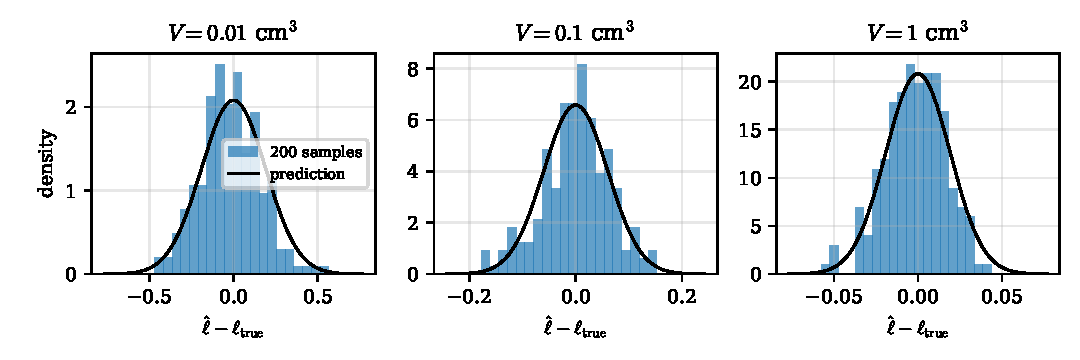
\includegraphics[width=\textwidth]{f_hist.pdf}
\caption{Distribution of $\hat\ell - \ell_{\mathrm{true}}$ over 200 samples (true $D_x = 10$), with the predicted Gaussian of standard deviation $1/\sqrt{\mathcal I}$. Note the shrinking horizontal scale as $V$ grows.}\label{fig:hist}
\end{figure}

\begin{figure}[h]
\centering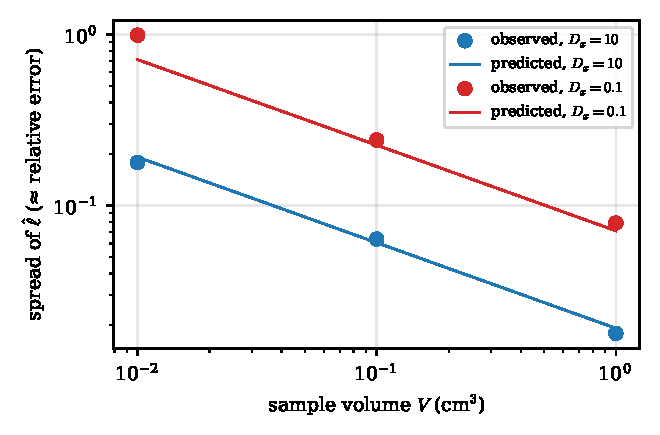
\includegraphics[width=0.62\textwidth]{f_scaling.pdf}
\caption{Observed spread (dots) and predicted spread (lines) versus sample volume. The lines have slope $-1/2$: ten times more sample gives about three times less error.}\label{fig:scaling}
\end{figure}

\paragraph{What we see.}
\begin{itemize}
\item \textbf{For $D_x = 10$, theory and experiment agree throughout.} The estimates are unbiased, and the observed spread matches the prediction within the statistical uncertainty of 200 samples. The relative error is about $19\%$, $6\%$ and $2\%$ for roughly $200$, $2000$ and $20{,}000$ droplets.
\item \textbf{$D_x = 0.1$ is harder.} For the same number of droplets, the error is about five times larger, because weak broadening changes the distribution less. With about $3400$ or $34{,}000$ droplets, the observed spread is within about $10\%$ of the prediction.
\item \textbf{The prediction fails when the information is very low.} At $D_x = 0.1$ with only about $340$ droplets, the predicted error is $71\%$. The observed spread is $99\%$, the estimates are skewed toward small values, and 4 of 200 fits ran to the lower bound. The parabola picture of Section~\ref{sec:errorbar} assumes the loss is close to a parabola over the range of plausible values, and when the error is comparable to the value itself, it isn't. In that regime, the error bar from \eqref{eq:sd} should be treated as optimistic.
\item \textbf{The $1/\sqrt V$ law holds} (Figure~\ref{fig:scaling}).
\end{itemize}

\subsection{One sample: does its error bar tell the truth?}\label{sec:single}
Figure~\ref{fig:single} shows a single sample with $V = 0.1$ cm$^3$ and true $D_x = 10$. The fit gives $\hat D_x = 9.88$ after 9 iterations. The curvature error bar is $\mathrm{sd}(\hat\ell) = 0.061$, so the estimate is $9.88$ within a factor $e^{\pm0.061}$, i.e.\ $[9.30,\,10.50]$, which contains the truth. The deviance is indeed close to a parabola over this range.

\begin{figure}[h]
\centering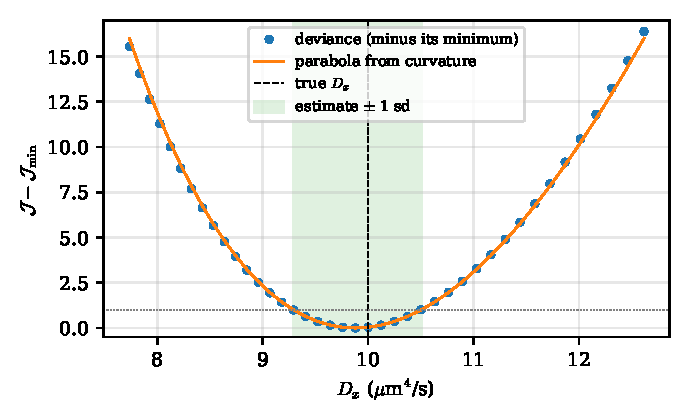
\includegraphics[width=0.62\textwidth]{f_single.pdf}
\caption{One sample: the deviance near its minimum (dots), the parabola implied by its curvature (line), and the resulting $\pm1$ sd interval (shaded), where the loss rises by 1 (dotted line).}\label{fig:single}
\end{figure}

One sample's error bar can't be judged in isolation. The meaningful test is: over many samples, does the interval $\hat\ell\pm\mathrm{sd}$ contain the truth about $68\%$ of the time, and $\hat\ell\pm2\,\mathrm{sd}$ about $95\%$ of the time, as a Gaussian error bar should? Figure~\ref{fig:errorbars} shows the first 40 samples: 27 of 40 intervals (68\%) contain the truth. Table~\ref{tab:coverage} gives the full results.

\begin{figure}[h]
\centering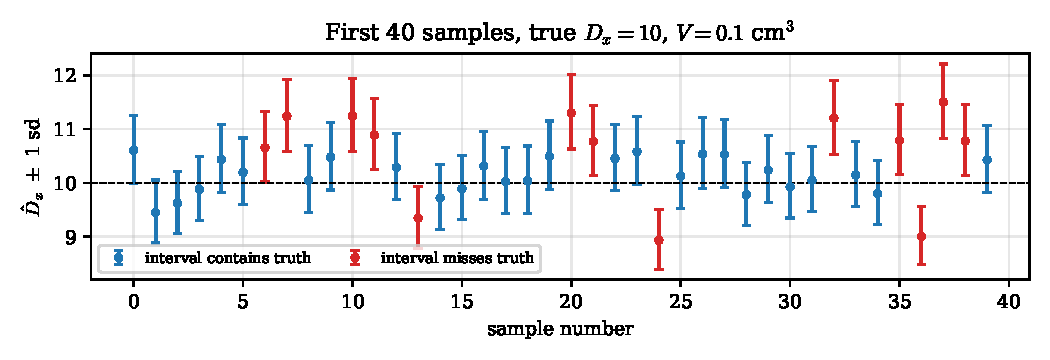
\includegraphics[width=\textwidth]{f_errorbars.pdf}
\caption{Estimates and their single-sample $\pm1$ sd error bars for the first 40 samples. About two-thirds of the intervals should contain the truth (blue), and about one-third should miss it (red).}\label{fig:errorbars}
\end{figure}

\begin{table}[h]
\centering\small
\begin{tabular}{@{}rrrrrr@{}}
\toprule
true $D_x$ & $V$ (cm$^3$) & observed spread & mean single-sample sd & within $\pm1$ sd & within $\pm2$ sd\\\midrule
10 & 0.01 & 0.179 & 0.192 & 71\% & 97\%\\
10 & 0.1 & 0.064 & 0.061 & 69\% & 93\%\\
10 & 1 & 0.018 & 0.019 & 72\% & 97\%\\
0.1 & 0.01 & 0.990 & 0.758 & 67\% & 95\%\\
0.1 & 0.1 & 0.241 & 0.228 & 62\% & 94\%\\
0.1 & 1 & 0.079 & 0.071 & 64\% & 91\%\\\midrule
\multicolumn{4}{r}{ideal (Gaussian)} & 68\% & 95\%\\\bottomrule
\end{tabular}
\caption{Do single-sample error bars tell the truth? Fraction of 200 samples whose interval contains the true value.}\label{tab:coverage}
\end{table}

The single-sample error bars are accurate: on average they match the scatter actually seen across samples, and they contain the truth about as often as they should. For $D_x = 0.1$ they are slightly optimistic, by roughly $5$--$10\%$, which shows up as coverage a few points below ideal. So with synthetic data we have confirmed the tool we will rely on for real data, where only one sample is available.

\subsection{The detection limit}\label{sec:cutoff}
Finally, we repeated the experiment with detection limits $\rdet = 1$, $2$ and $3\um$, dropping all bins below the limit. For $D_x = 0.1$ we used $V = 1$ cm$^3$, so that the no-cutoff error is small enough to see the effect clearly.

\begin{table}[h]
\centering\small
\begin{tabular}{@{}lrrrrrr@{}}
\toprule
& \multicolumn{3}{c}{$D_x = 10$, $V = 0.1$ cm$^3$} & \multicolumn{3}{c}{$D_x = 0.1$, $V = 1$ cm$^3$}\\
cutoff & droplets seen & predicted & observed & droplets seen & predicted & observed\\\midrule
none & 2053 & 0.061 & 0.064 & 34387 & 0.071 & 0.079\\
$1\um$ & 1977 & 0.063 & 0.060 & 31437 & 0.122 & 0.119\\
$2\um$ & 1870 & 0.066 & 0.069 & 28072 & 0.247 & 0.266\\
$3\um$ & 1705 & 0.071 & 0.070 & 23879 & 0.352 & 0.561\\\bottomrule
\end{tabular}
\caption{Spread of $\hat\ell$ (approximately relative error) with a detection limit, 200 samples each.}\label{tab:cutoff}
\end{table}

\begin{figure}[h]
\centering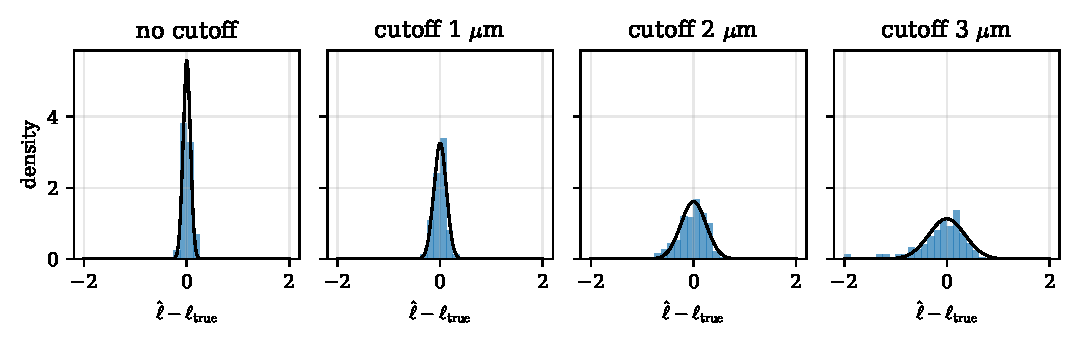
\includegraphics[width=\textwidth]{f_cutoff.pdf}
\caption{Distribution of $\hat\ell - \ell_{\mathrm{true}}$ for $D_x = 0.1$, $V = 1$ cm$^3$, as the detection limit rises, with the predicted Gaussian.}\label{fig:cutoff}
\end{figure}

\begin{itemize}
\item \textbf{For $D_x = 10$ the cutoff barely matters.} Strong broadening reshapes the whole distribution, so seeing most of it is enough. Even a $3\um$ cutoff, which hides 17\% of the droplets, raises the error only from $6.1\%$ to $7.1\%$.
\item \textbf{For $D_x = 0.1$ the cutoff is severe.} A $2\um$ cutoff hides only 18\% of the droplets but more than triples the error, from $7\%$ to about $25\%$. With a $3\um$ cutoff the observed spread is about eight times the no-cutoff value, and the estimates are skewed and the curvature error bar is optimistic: predicted $35\%$, observed $56\%$, the same low-information breakdown seen in Section~\ref{sec:mc}. When turbulence is weak, its fingerprint is mostly fine structure near the activation size of about $1\um$, which is exactly what the cutoff hides.
\end{itemize}
So whether $D_x$ can be recovered from instrument data depends strongly on where the detection limit sits relative to the activation region, and on how large $D_x$ is.

%==================================================================
\section{Summary}
%==================================================================
\begin{itemize}
\item Sampling a small volume of a well-mixed chamber gives unbiased but noisy counts. Each bin's count is Poisson with mean $\mu_k = V\int_{\text{bin}}N\,\dd x$, and different bins are independent.
\item Maximum likelihood gives the Poisson deviance \eqref{eq:dev} as the loss. Unobserved bins (below the detection limit) are left out, not set to zero.
\item The adjoint machinery is unchanged except for $\mathbf{g} = V\Hm^\top[2(1 - c_k/\mu_k)]$.
\item The curvature of the loss at its minimum gives a single-sample error bar, $\mathrm{sd}(\hat\ell)\approx\sqrt{2/\J''}$. Over many synthetic samples, these error bars match the observed scatter and contain the truth about 68\% of the time, as they should.
\item Precision improves as $1/\sqrt{V}$. Small $D_x$ is intrinsically harder to pin down, and a detection limit above the activation size makes it much harder. When the information is low, the estimates become skewed and the error bars become optimistic.
\end{itemize}
Natural next steps are to generate the truth on a finer grid than the fit (so that numerical errors no longer cancel), to add noise that is correlated across bins or larger than Poisson, and to estimate additional parameters alongside $D_x$.

\appendix
%==================================================================
\section{Parameter values}\label{app:params}
%==================================================================
\begin{center}\small
\begin{tabular}{@{}>{\raggedright\arraybackslash}p{4.6cm}>{\raggedright\arraybackslash}p{4.8cm}>{\raggedright\arraybackslash}p{5.6cm}@{}}
\toprule
Quantity & Value & Note\\\midrule
Temperature, pressure & $288$ K, $1000$ hPa & \\
Supersaturation & $s = 0.09\%$ & \\
Growth coefficient & $a = 205.8\um^2$/s & $\dd(r^2)/\dd t = a\,s$ for large droplets\\
Köhler parameters & $A_k = 1.128\times10^{-3}\um$, $B_k = 3.650\times10^{-4}\um^3$ & NaCl, dry radius $0.065\um$\\
Removal constant & $k = 1.210\times10^{-4}\ \mu$m$^{-2}$s$^{-1}$ & Stokes fall speed / chamber height ($1$ m)\\
Injection rate & $\Fin = 100$ cm$^{-3}$s$^{-1}$ & \\
Grid & $8000$ cells, $\Delta x = 0.1125\um^2$, $r\in[0.0325, 30]\um$ & \\
Bins & $8$ cells per bin, width $0.9\um^2$, $K = 1000$ & \\
Sample volumes & $V = 0.01$, $0.1$, $1$ cm$^3$ & \\
Monte Carlo & 200 samples per case & starting guess $D_x = 1$, bounds $[10^{-3},10^3]$\\\bottomrule
\end{tabular}
\end{center}

\end{document}
